\documentclass[twocolumn]{IEEEtran}
\usepackage{graphicx}
\usepackage[utf8x]{inputenc}
\usepackage{times}
\usepackage{amssymb,amsfonts}
\usepackage{pict2e}
\usepackage{float}
\usepackage[all]{xy}
\usepackage{graphics,graphicx,color,colortbl}
\usepackage{subfigure}
\usepackage{wrapfig}
\usepackage{multicol}
\usepackage{cite}
\usepackage{url}
\usepackage[tbtags]{amsmath}
\usepackage{amsmath,amssymb,amsfonts,amsbsy}
\usepackage{bm}
\usepackage{listings}
\usepackage{algorithm}
\usepackage{algorithmic}
\usepackage[centerlast, small]{caption}
\usepackage[colorlinks=true, citecolor=blue, linkcolor=blue, urlcolor=blue, breaklinks=true]{hyperref}
\hyphenation{ele-men-tos he-rra-mi-en-ta cons-tru-yen trans-fe-ren-ci-a co-rres-pon-dien-tes co-rres-pon-de}

\begin{document}
\title{Caracterización experimental de substratos dieléctricos}
%Experimental Characterization of dielectric substrates
\author{David Ricardo Martínez Hernández Código: $261931$\\
Jairo Andrés Neuta Bernal Código: $261227$}
\maketitle
\markboth{Universidad Nacional de Colombia}{}
\floatname{algorithm}{Algoritmo}

\begin{abstract}
This document presents a procedure for the characterization of a dielectric substrate which includes fabrication, measurement and calculation to obtain the dielectric constant and loss tangent of the material is applicable to the characterization of sample in the band 2-3 GHz with permittivity values in the ranges 2-10. A  Microstrip system in short circuit and open circuit  are manufactured above the thereof dielectric substrate ,  with SMA connector that allows its connection to the Vector Network Analyzer which provides  1- port parameter of the system. This parameter is used to obtain the material parameters sought.

\end{abstract}

\begin{keywords}
 Amplitud, Coeficiente de reflexión, Conector SMA, Constante de pérdidas, Constante dieléctrica, Fase, FR4, Impedancia Característica, Impedancia de Entrada, Línea de transmisión, Parámetros S, Sistema Microstrip, Sustrato Dieléctrico, VNA.
\end{keywords}

\section{Introducción}
\noindent
El proceso de caracterización de un sustrato dieléctrico, corresponde a un factor de vital importancia en el mundo actual, ya que muchas de las aplicaciones tecnológicas, dependen de las propiedades electromecánicas y del comportamiento que presentan los materiales dieléctricos a altas frecuencias y que influencian de manera directa el desempeño de dispositivos electrónicos tales como acopladores, resonadores y antenas entre otros.\\
En el momento de realizar la caracterización de un sustrato dieléctrico, se evidencian diversos factores que muchas veces no son controlables y dependen únicamente de las condiciones en las que se desarrolle la prueba de caracterización e indispensablemente de las herramientas tecnológicas con las que se cuente. Estos parámetros constituyen el éxito, prestigio o fracaso de un método empleado para la caracterización del sustrato dieléctrico. En la bibliografía actual existen distintos métodos de caracterización de sustratos dieléctricos, los cuales se ven diferenciados unos de otros, por aspectos tales como; el uso de instrumentación especifica, el costo tecnológico de la misma, el rango de frecuencias en las que se puede evaluar, la facilidad de construcción e implementación del método, la precisión en la medición, el acople adecuado entre dispositivos de medida y la capacidad de repetir tantas veces sea necesario el método de caracterización y obtener resultados similares bajo condiciones similares.\\
La línea de transmisión conocida como sistema microstrip,  que se construirá sobre el sustrato dieléctrico propuesto (FR4), pertenece  a la categoría de las líneas de transmisión de placas paralelas  y  normalmente es el tipo de líneas de transmisión  más utilizado en la electrónica actual por su fácil implementación, bajo costo y en virtud por su  diseño más compacto en comparación de otros casos como lo puede ser: las líneas de transmisión coaxial. Se caracteriza por presentar fuertes fugas de radiación de campo electromagnético en el aire ya que este no se encuentra confinado totalmente al dieléctrico, lo que se traduce en pérdidas de energía.  Adicionalmente como las velocidades de fase son diferentes, se produce dispersión de la onda transmitida, también es susceptible a captar gran cantidad de ruido perturbando así la onda transmitida. Es importante mencionar que debido al efecto de borde presente en la línea de transmisión, la permitividad relativa efectiva ($\epsilon _{ref}$) es menor que la permitividad relativa ($\epsilon _r$) del sustrato dieléctrico y adicionalmente si  la permitividad relativa $\epsilon _r$ crece, la impedancia característica ($Z_0$) disminuye.\\
En este documento se presenta el desarrollo de la metodología de caracterización de un sustrato dieléctrico en general, empleado en un sistema microstrip. Con el objetivo de obtener experimentalmente los valores de constante dieléctrica del sustrato caracterizado y adicionalmente las pérdidas dieléctricas del mismo.  En la primera parte del documento se presenta el diseño del sistema a partir del método propuesto, seguido se presenta la medición técnica desarrollada, donde se muestra el procedimiento de cálculos y de simulación para validar el método propuesto,  posteriormente se presentan los resultados y análisis de los datos experimentales y finalmente a manera de conclusiones se presentan los aspectos fundamentales en el método de caracterización del sustrato desarrollado.

\section{Marco Teórico}
\noindent
El sistema microstrip consiste en una franja de material conductor generalmente de cobre con  un ancho W , un largo L y un espesor T definidos, que se encuentra  separada una distancia H de un plano de tierra de dimensiones muchísimo mayores  por medio de un material dieléctrico.  Este material  o sustrato dieléctrico representa uno de los componentes  más importantes  que caracterizan un sistema microstrip;  estas características  varían de acuerdo al  material a implementarse en la línea de transmisión,  es  decir ; a su espesor H, su  permitividad relativa $\epsilon _r$ y la constante de pérdidas característica,  estos parámetros definen el funcionamiento general de la línea de transmisión Fig. \ref{fig1}\footnote{Imagen tomada de \cite{page1}}.
\begin{figure}[]
	\centering
		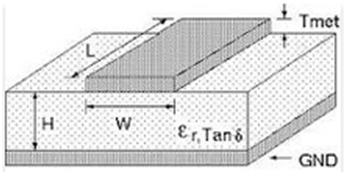
\includegraphics[scale=0.6]{line.png}
	\caption{Geometría de una Microstrip Line.}
	\label{fig1}
\end{figure}

\subsection{FR4 (Resina Epoxi/Fibra de Vidrio)}
\noindent
Es un material fabricado a base de fibra de vidrio, el cual a su vez está constituido por capas tejidas de fibra de vidrio impregnadas con resina epóxica resistente a las llamás. Las letras ``FR'' en la designación del material indican ``retardante de llama'' (\textit{Flame Retardant}). El material tiene un espesor Standard de ($1.6mm$) y consta de $8$ capas de Prepeg y una de cobre de $35$ micrones ($1 Oz/ft2$). Las capas de Prepeg y el laminado de cobre se prensan bajo presión y temperatura controladas para conformar el material final que se utilizará en los procesos de fabricación.\\
Este es uno de los materiales más usados en la fabricación de circuitos impresos, en especial en tecnología de microcintas debido a las buenas características eléctricas y mecánicas que presenta.\\
Sus principales características son:
\begin{itemize}
 \item Mecánicas:
\begin{itemize}
 \item Suficientemente rígidos para mantener los componentes.
 \item Fácil de taladrar.
 \item Sin problemás de laminado.
\end{itemize}
 \item Químicas:
\begin{itemize}
 \item Metalizado de los taladros.
 \item Retardante de las llamás.
 \item No absorbe demásiada humedad.
\end{itemize}
 \item Térmicas:
\begin{itemize}
  \item Disipa bien el calor.
 \item Coeficiente de expansión térmica bajo para que no se rompa.
 \item Capaz de soportar el calor en la soldadura.
 \item Capaz de soportar diferentes ciclos de temperatura.
\end{itemize}
 \item Eléctricas:
\begin{itemize}
  \item Constante dieléctrica baja para tener pocas pérdidas.
 \item Punto de ruptura dieléctrica alto.	
\end{itemize}
\end{itemize}

%$$ \epsilon _{r,eff}  = \left\{ \begin{array}{l} \frac{{\epsilon _r  + 1}}{2} + \frac{{\epsilon _r  - 1}}{2}\left[ {\frac{1}{{\sqrt {1 + 12\frac{h}{w}} }} + 0.04\left( {10 - \frac{w}{h}} \right)} \right]^2 \ \ \frac{w}{h} \le 1.0 \\ 
% \frac{{\epsilon _r  + 1}}{2} + \frac{{\epsilon _r  - 1}}{{2\sqrt {1 + 12\frac{h}{w}} }}\ \ \frac{w}{h} \ge 1.0 \\ 
% \end{array} \right. $$ %Ecuación epsilon relativo
%$$ Z_0  = \left\{ \begin{array}{l}
% \frac{{60}}{{\sqrt {\epsilon _{r,eff} } }}\ln \left( {\frac{{8h}}{w} + \frac{w}{{4h}}} \right)\ \ \frac{w}{h} \le 1.0 \\ 
% \frac{{120\pi }}{{\sqrt {\epsilon _{r,eff} } \frac{w}{h} + 1.393 + 0.667\ln \left( {\frac{w}{h} + 1.444} \right)}}\ \ \frac{w}{h} \ge 1.0 \\ 
% \end{array} \right. $$%Ecuación Impedancia caracteristica

%\begin{equation}
% \frac{{\Delta w}}{t} = \frac{{1.0}}{\pi }\ln \left( {\frac{{4e}}{{\sqrt {\left( {\frac{t}{h}} \right)^2  + \left( {\frac{{1/\pi }}{{w/t + 1.1}}} \right)^2 } }}} \right)
%\label{ecu1}%Ecuación de delta w
%\end{equation}

%\begin{equation}
% \frac{{\Delta l}}{h} = 0.412\frac{{er + 0.3}}{{er - 0.258}}\frac{{w + 0.264h}}{{w + 0.8h}}
%\label{ecu2}%Ecuación de delta h
%\end{equation}
%{\tiny{
%$$ \alpha_c \left( {Np/m} \right) = \left\{ \begin{array}{l}
 %\frac{{R_s }}{{2\pi }}\frac{{\left( {\frac{{8.0h}}{w} - \frac{w}{{4h}}} \right)\left( {1.0 + \frac{h}{w}\left( {1 + \frac{{\partial w}}{{\partial t}}} x\right)} \right)}}{{hZ_0 e^{\frac{{Z_0 }}{{60}}} }} \ \frac{w}{h} \le 1.0 \\ 
 %\frac{{Z_0 R_s }}{{14400\pi ^2 h}}\left[ {1.0 + \left( {\frac{h}{w}} \right)^2 0.44 + 6.0\left( {1.0 - \frac{h}{w}} \right)^5 } \right]\left( {1.0 + \frac{w}{h} + \frac{{\partial w}}{{\partial t}}} \right) \ \frac{w}{h} \ge 1.0 \\ 
% \end{array} \right.
%$$}}%Ecuación de alfa por conducción
%\noindent
%Donde
%$$ \frac{{\partial w}}{{\partial t}} = \left\{ \begin{array}{l}
% \frac{{1.0}}{\pi }\ln \left( {\frac{{4.0\pi w}}{t}} \right)\ \ \frac{w}{h} \le \frac{1}{{2\pi }} \\ 
% \frac{{1.0}}{\pi }\ln \left( {\frac{{20h}}{t}} \right)\ \ \frac{w}{h} \ge \frac{1}{{2\pi }} \\ 
% \end{array} \right. $$ %Derivadas de alfa

%\begin{equation}
% \alpha _d \left( {Np/m} \right) = \pi \frac{{\frac{{\epsilon _{r,eff}  - 1}}{{\epsilon _r  - 1}}\tan \delta }}{{\lambda _0 /\sqrt {\epsilon _{r,eff} } }}
%\label{ecu3}%Alfa por dieléctrico
%\end{equation}

\section{Metodología}
\noindent
Para el desarrollo del proyecto se ha propuesto  un método  de caracterización de  sustratos dieléctricos  a modo general, para  el que se ha planteado un ambiente en el que se tiene dos sistemás Microstrip sobre un mismo sustrato dieléctrico desconocido, uno terminado en corto circuito y el otro terminado en circuito abierto. Para el cual no se conoce el valor de su permitividad relativa y de la tangente de pérdidas del material dieléctrico de estudio, los únicos datos conocidos hacen parte de la información que se ha suministrado como especificaciones del proyecto, esta información corresponde al  rango de posibles valores en que se encuentra la permitividad $\epsilon _r$ ($2$ a $20$), el rango de frecuencias de medición (2-3 GHz) y la pérdidas dieléctricas del material ($0.001-0.1$). El objetivo del método trabajado es el de encontrar una buena aproximación del valor de $\epsilon _r$ y $tan \delta$ del sustrato dieléctrico en el que se albergan los dos sistemás Microstrip.\\
Con el método empleado se ha fijado de manera conveniente los valores de $W$ y $L$, con el fin de que las dimensiones seleccionadas permitan una construcción práctica y sencilla de los sistemás Microstrip. (Ver  Fig. \ref{fig1}).\\
La fabricación de los sistemás Microstrip se ha desarrollado teniendo en cuenta la medición de parámetros físicos como la estimación del espesor $H$ del sustrato dieléctrico y del ancho $W$ de la línea de transmisión se midieron utilizando un calibrador Pie de Rey digital TABLA \ref{tab1}
\begin{table}[H]
	\centering
\begin{tabular}{|c|c|c|}\hline
\textbf{Parámetros} & \textbf{Linea Corto Circuito} & \textbf{Linea Circuito Abierto} \\ \hline
\textbf{W} & $4.5mm$ & $4.5mm$ \\ \hline
\textbf{L} & $60.61mm$ & $58.81mm$ \\ \hline
\textbf{H} & $0.711mm$ & $0.711mm$ \\ \hline
    \end{tabular}
	\caption{Parámetros medidos con el calibrador}
	\label{tab1}
\end{table}

\subsection{Simulaciones}
\noindent
\begin{figure}[H]
	\centering
		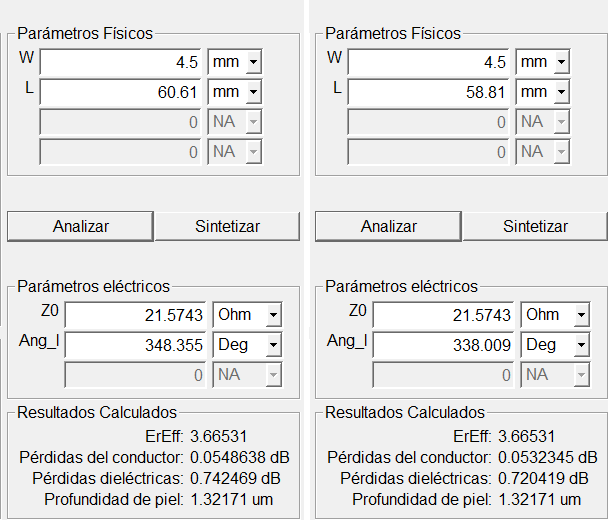
\includegraphics[scale=0.5]{simula2.png}
	\caption{Simulación en Qucs de los parámetros de las líneas.}
	\label{fig2}
\end{figure}
\noindent
Los datos obtenidos en la simulación que se muestran en la Fig. \ref{fig2}, se simularon teniendo en cuenta los parámetros del sustrato con los siguientes valores: $H=0.711mm$, $\epsilon _r = 4.34$, $tan \delta = 0.03$ y  parámetros del componente a una frecuencia de $f=2.5GHz$.\\
Con los parámetros $S[1,1]$ obtenidos previamente en la simulación de Qucs, calcularemos la $tan \delta$ y el $\alpha _c$ en un algoritmo desarrollado en Matlab (\textit{CttProp.m}). Estos resultados se encuentran en Fig. \ref{fig3} y Fig. \ref{fig4}.\\
En la Fig. \ref{fig3} no existe diferencia en el $\alpha _c$, dado que es el mismo para ambos casos. Es importante determinar este parámetros porque con este se facilita determinar el valor de las perdidas por dieléctrico mediante el uso de ecu. (\ref{ecu1}).
\begin{equation}
 \alpha _d \left( {Np/m} \right) = \pi \frac{{\frac{{\epsilon _{r,eff}  - 1}}{{\epsilon _r  - 1}}\tan \delta }}{{\lambda _0 /\sqrt {\epsilon _{r,eff} } }}
\label{ecu1}%Alfa por dieléctrico
\end{equation}

\begin{figure}[]
	\centering
		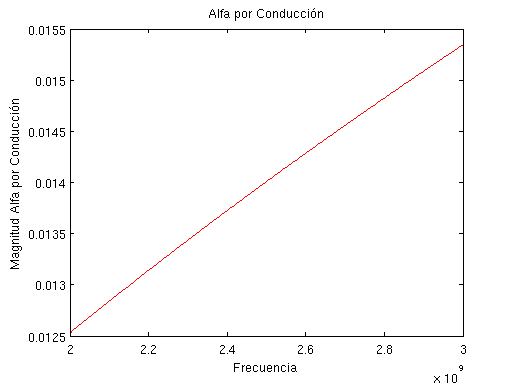
\includegraphics[scale=0.6]{alfacsim.png}
	\caption{Gráfica obtenida de la simulación para el valor del Alfa por Conducción.}
	\label{fig3}
\end{figure}
\noindent
Es importante mencionar que el valor de $tan \delta$ Fig. \ref{fig4} de la línea en terminada en corto circuito y circuito abierto, rojo y azul respectivamente.
\begin{figure}[]
	\centering
		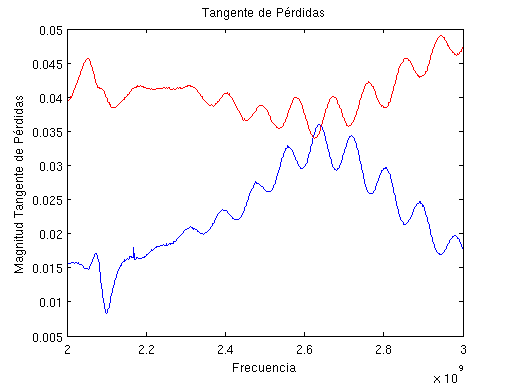
\includegraphics[scale=0.6]{losstangsim.png}
	\caption{Gráfica obtenida de la simulación para el valor de la tangente de Pérdidas.}
	\label{fig4}
\end{figure}

\section{Resultados de la Medición}
\noindent
Dados los resultados obtenidos por medio del \textbf{VNA or the Rohde \& Schwarz} se realizo un programa en Matlab para determinar de manera más rápida los valores deseados y así poder interpretar los resultados obtenidos.\\
Como los valores obtenidos en los archivos \textit{g14ol.txt} y \textit{g14sl.txt} se encontraban en columnas de frecuencia, magnitud en $dB$ y fase en grados, se realizo una conversión a $Nepers/m$ y se trabajo con la fase dada en grados.
\begin{figure}[]
	\centering
		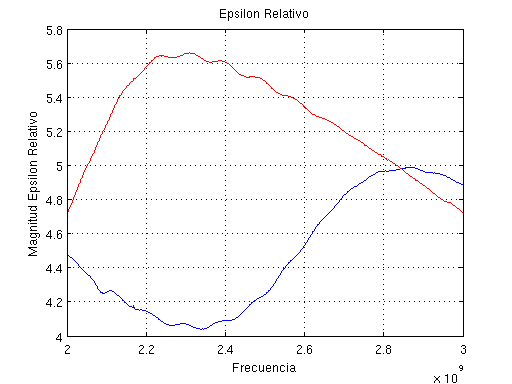
\includegraphics[scale=0.6]{epsilonrelative.png}
	\caption{Gráfica de los datos de Epsilon Relativo obtenidas en la práctica.}
	\label{epre}
\end{figure}
\noindent
En la Fig. \ref{epre} se encuentran dos gráficas sobre puestas que representan el $\epsilon _r$ para las líneas en corto circuito y circuito abierto, rojo y azul respectivamente.\\
Para el caso de la línea terminada en circuito abierto se puede observar que para el rango de frecuencias de muestreo el valor del $\epsilon _r$ oscila entre dos valores ($4.1-5$), para el $\epsilon _{rmin}$ se encuentra a una frecuencia aproximadamente de $2.35 GHz$ y su valor máximo $\epsilon _{rmax}$ a $2.85GHz.$. Se puede observar que a la frecuencia de corte de $2.5GHz$ se obtiene un valor de $\epsilon _r =4.3$.\\
Para la línea terminada en corto circuito se puede observar que para el rango de frecuencias de muestreo el valor del $\epsilon _r$ oscila entre dos valores ($4.75-5.65$), para el $\epsilon _{rmin}$ se encuentra en los valores límites del rango de medición y su valor máximo $\epsilon _{rmax}$ a $2.3GHz.$. Se puede observar que a la frecuencia de corte de $2.5GHz$ se obtiene un valor de $\epsilon _r =5.5$.\\
Observando las dos curvas de la Fig. \ref{epre}, se encontraron resultados muy diferentes aunque se haya trabajado sobre el mismo substrato dieléctrico, es evidente que los resultados varíen cuando se trabaje con una línea terminada en corto circuito o circuito abierto. Una de las razones a considerar para obtener esta diferencia en los resultados es la generada por un $\Delta W$ que se genero por el proceso de fabricación no tan preciso. Además influyo la distancia que existió entre el final de la línea y el borde del sistema Microstrip.
\begin{figure}[]
	\centering
		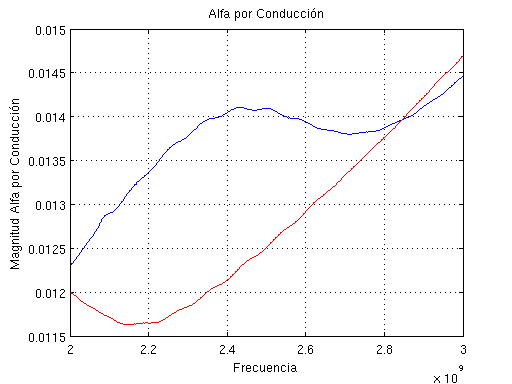
\includegraphics[scale=0.6]{alfac.png}
	\caption{Gráfica de los datos de Alfa por Conducción obtenidas en la práctica.}
	\label{alfac}
\end{figure}
\noindent
Continuando con la misma convención de colores para cada una de las líneas analizadas se puede observar en la Fig. \ref{alfac} que para el caso de la línea terminada en corte circuito se encontro un comportamiento casi lineal creciente en el rango de frecuencias de $2.2-3 GHz$. El valor mínimo del $\alpha _{cmin}=0.0115$ corresponde a una frecuencia de $2.2GHz$ y un valor máximo de $\alpha _{cmax}=0.0145$ par una frecuencia de $3GHz$, es importante mencionar que para la frecuencia de corte $\alpha _c=0.0125$.\\
Para el caso de la línea terminada en circuito abierto se puede observar tiene una valor mínimo de $\alpha _{cmin}=0.0124$ a una frecuencia de $2GHz$ y un valor máximo $\alpha _{cmax}=0.0145$ a una frecuencia de $3GHz$, para el caso de la frecuencia de corte el valor es de $\alpha _c= 0.014$. Adicionalmente se observa que en la Fig. \ref{epre} y Fig. \ref{alfac} se observa que las curvas para cada una de las líneas tienen un punto de corte aproximadamente en $2.85GHz$.
\begin{figure}[]
	\centering
		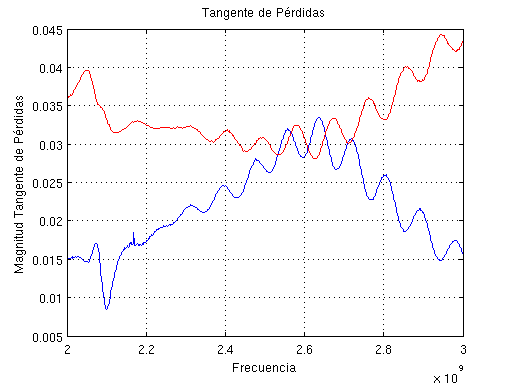
\includegraphics[scale=0.6]{losstang.png}
	\caption{Gráfica de los datos de la tangente de pérdidas ($tan \delta$) obtenidas en la práctica.}
	\label{tanloss}
\end{figure}
\noindent
Para la Fig. \ref{tanloss} se puede observar que las perdidas generas por el dieléctrico para la línea roja terminada en corto circuito sus perdidas son mayores en todo el rango de frecuencias excepto en el intervalo de $2.55-2.65 GHz$, con respecto a la línea azul terminada en circuito abierto.

\section{Método de adicional para caracterización de sustratos dieléctricos}
\noindent
El método seleccionado como referencia para desarrollar la caracterización de los sustratos propuestos, es el descrito en el documento titulado ``\cite{benavides} DISEÑO E IMPLEMENTACIÓN DE UN AMPLIFICADOR DE MICROONDAS A 2.45 GHZ APLICANDO TÉCNICAS PARA EL MEJORAMIENTO DE LA GANANCIA Y LA FIGURA DE RUIDO.'' En la sección 2 de este documento, se expone dos técnicas de caracterización; la primera  se denomina  Resonador basado en tecnología de microcintas: esta técnica consiste en utilizar una línea de longitud definida como resonador, conectada a dos líneas laterales de alimentación, el otro método es el desarrollado por el Ing. Julián Herrera.


\section{Conclusiones}
\begin{itemize}
 \item Debido al proceso de fabricación el prototipo desarrollado para las líneas de transmisión trabajo cerca al límite, el cual esta al rededor de los $4.5mm$ en donde su comportamiento puede llegar a cambiar pasando de una línea de transmisión a una antena, es por eso que se cree que los resultados se ven influenciados por el ruido electromagnético presente en el ambiente.
 \item Al observar la Fig. \ref{epre} y la Fig. \ref{alfac} se puede deducir que sin importar si se esta trabajando con una línea terminada en corto circuito o en circuito abierto a una frecuencia de $2.85GHz$ se obtendra el mismo comportamiento es decir que para el caso del $\epsilon _r$ sera aproximadamente de $4.95$ y un $\alpha _c$ de $0.014$ para dicha frecuencia.
 \item Al observar la Fig. \ref{tanloss} que representa los datos experimentales se encuentra que en el intervalo de frecuencias de $2.55-2.65 GHz$ el promedio de las pérdidas para los dos casos de líneas es similar y se encuentra alrededor de $0.03$. Además observando las curvas obtenidas se puede concluir que tiene un comportamiento similar, las variaciones máximas oscilan en un $0.005$ del valor experimental con respecto al teórico.
 \item Se encontró que para el caso de la Fig. \ref{fig3} la gráfica de la línea terminada en corto circuito de los datos experimentales Fig. \ref{alfac} trato de seguir el mismo comportamiento de los datos simulados. Partiendo y finalizando aproximadamente en los mismos valores correspondientes a la atenuación por dieléctrico dentro del rango de frecuencias de medición, es valido mencionar que para el caso de la línea terminada en circuito abierto el comportamiento varia durante todo el intervalo en comparación con la gráfica obtenida con los datos simulados.
 \item Como se supuso que el $\epsilon _{rteorico}=4.3$ y corresponde a una linea horizontal durante todo el intervalo se encontró que los datos experimentales poseen una variación de $\pm 0.7$, para el caso de la línea terminada en circuito abierto y para la línea terminada en corto circuito posee una variación de $\pm 1.4$.
 \item Los valores tanto de $\epsilon _r$ y de la $tan \delta$ experimentales a la frecuencia de resonancia son muy cercanos a los valores simulados para la línea terminada en circuito abierto. En el caso de la línea terminada en corto circuito se aleja una unidad por encima del valor esperado.
\end{itemize}

\bibliographystyle{ieeetran}
\begin{thebibliography}{99}

\bibitem{benavides} Benavides Cerpa, Orlando Andrés.
{\em "`Diseño e implementación de un amplificador de microondas a 2.45 ghz aplicando técnicas para el mejoramiento de la Ganancia y la figura de ruido."'}
Tesis de Pregrado del 2010.

\bibitem{chen} Chen, Chi-Tsong.
{\em "`Analog and Digital Control System Desing: Transfer-Function, State, Space and Algebraic Methods"'}.
Saunders College Publishing, 1993.

\bibitem{sadiku} Sadiku, Matthew N.O.
{\em "`Elementos de electromagnetismos."'}
Tercera Edición. Oxford University Press, 2002. pag: 524-527.

\bibitem{page1} \url{http://www.ece.ncsu.edu/erl/html2/papers/steer/1990/riedell_steer_apr_1990.pdf}

\end{thebibliography}
\end{document}